% How a question gets answered: who does what (LLM vs embedding model vs plain code).
% Build: cd docs && pdflatex how_it_works.tex && pdfcrop --margins 10 how_it_works.pdf how_it_works.pdf
%        && pdftoppm -png -r 150 -singlefile how_it_works.pdf how_it_works
\documentclass{article}
\usepackage[paperwidth=24cm,paperheight=40cm,margin=0.5cm]{geometry}
\pagestyle{empty}
\usepackage[T1]{fontenc}
\usepackage[utf8]{inputenc}
\usepackage[scaled]{helvet}
\renewcommand{\familydefault}{\sfdefault}
\usepackage{tikz}
\usetikzlibrary{arrows.meta}

\definecolor{llm}{HTML}{E67E22}
\definecolor{emb}{HTML}{27AE60}
\definecolor{code}{HTML}{1F5FAD}
\definecolor{db}{HTML}{5D6D7E}

\begin{document}\noindent
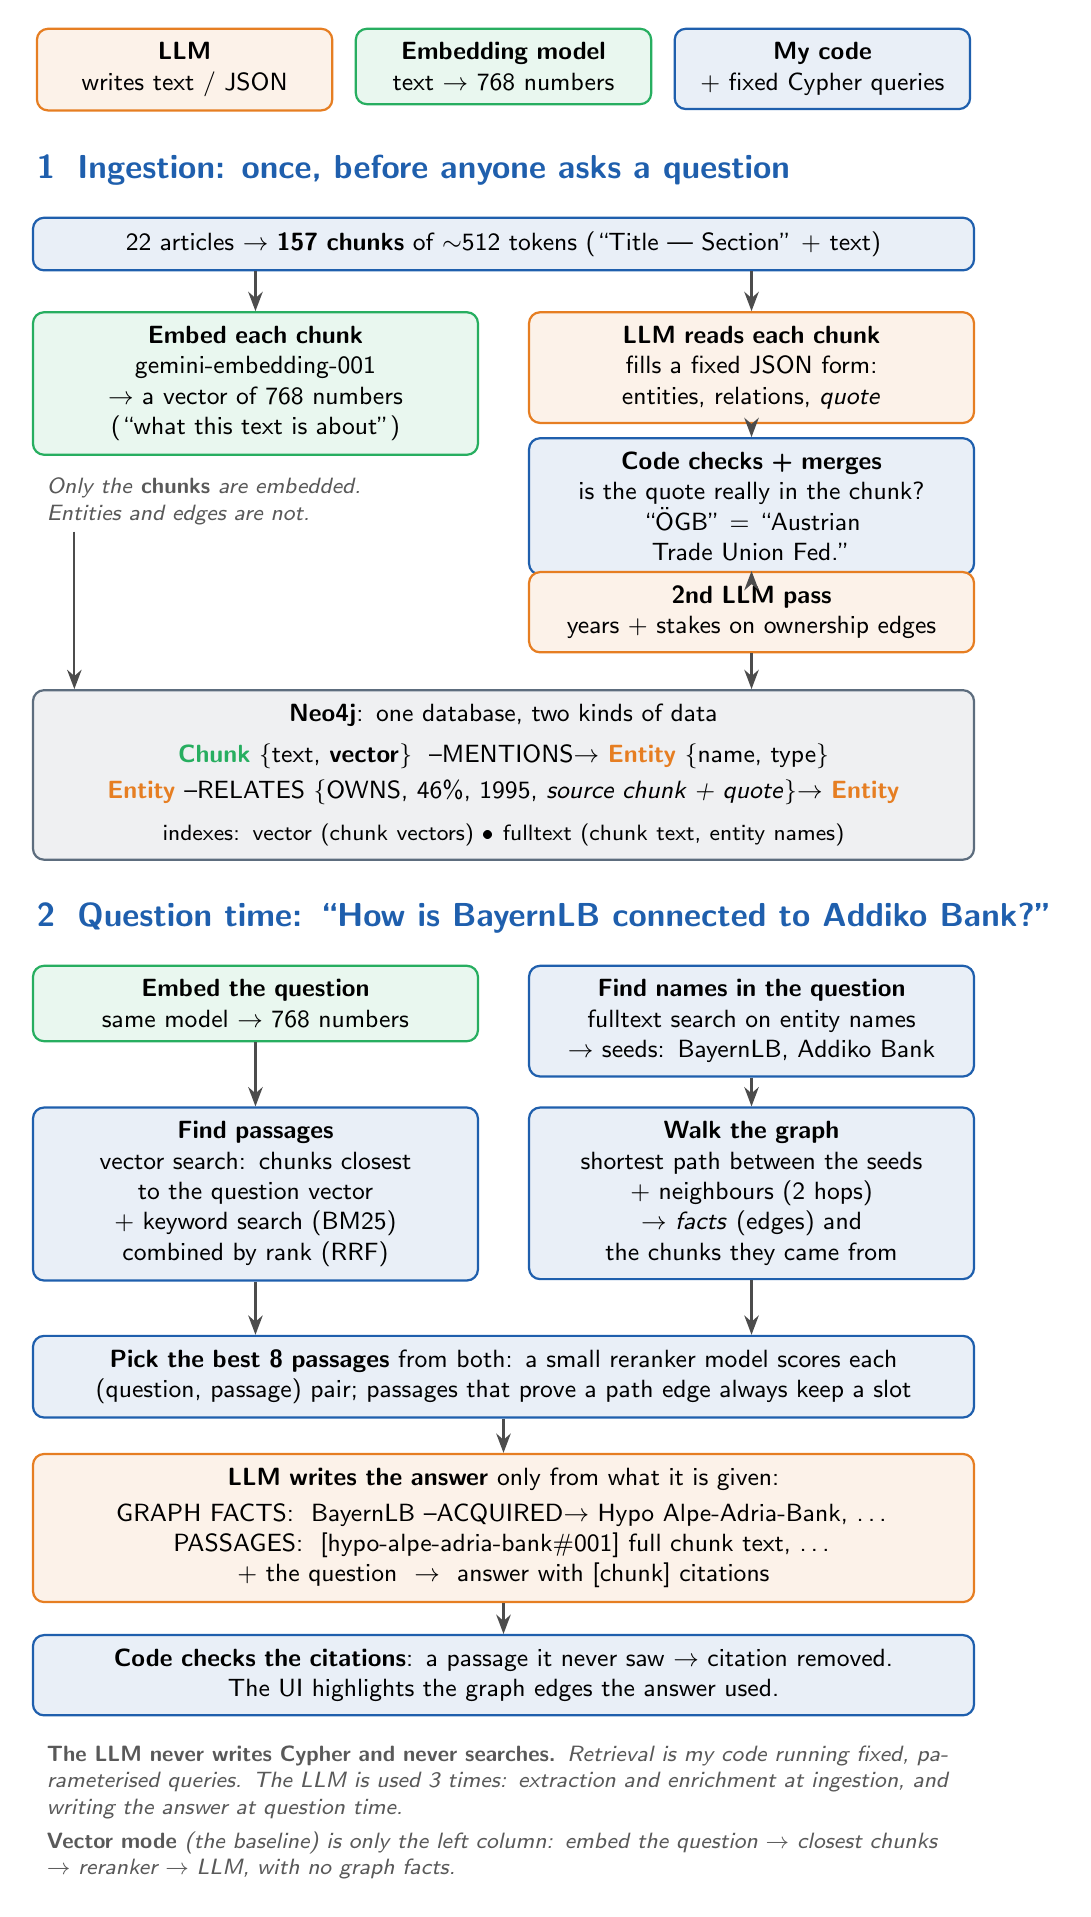
\begin{tikzpicture}[
    font=\small,
    box/.style={draw=#1, fill=#1!10, rounded corners, thick, align=center,
                text width=5.3cm, inner sep=5pt, anchor=north},
    wide/.style={box=#1, text width=11.6cm},
    small/.style={box=#1, text width=3.4cm},
    arr/.style={-{Stealth[length=7pt]}, thick, black!70},
    note/.style={font=\footnotesize\itshape, text=black!65, align=left},
    title/.style={font=\large\bfseries, text=code, anchor=north west},
  ]
  % columns: left centre x=0, right centre x=6.3, wide centre x=3.15

  % ---------------- legend ----------------
  \node[small=llm]  at (-0.9, 0) {\textbf{LLM}\\writes text / JSON};
  \node[small=emb]  at (3.15, 0) {\textbf{Embedding model}\\text $\to$ 768 numbers};
  \node[small=code] at (7.2, 0) {\textbf{My code}\\+ fixed Cypher queries};

  % ---------------- part 1: ingestion ----------------
  \node[title] at (-2.9, -1.5) {1 \;Ingestion: once, before anyone asks a question};

  \node[wide=code] (chunk) at (3.15, -2.4)
    {22 articles $\to$ \textbf{157 chunks} of $\sim$512 tokens (``Title | Section'' + text)};

  \node[box=emb] (embed) at (0, -3.6)
    {\textbf{Embed each chunk}\\gemini-embedding-001\\$\to$ a vector of 768 numbers\\(``what this text is about'')};
  \node[note, text width=5.3cm, anchor=north] at (0, -5.6)
    {Only the \textbf{chunks} are embedded.\\Entities and edges are not.};

  \node[box=llm] (extract) at (6.3, -3.6)
    {\textbf{LLM reads each chunk}\\fills a fixed JSON form:\\entities, relations, \emph{quote}};
  \node[box=code] (check) at (6.3, -5.2)
    {\textbf{Code checks + merges}\\is the quote really in the chunk?\\``ÖGB'' = ``Austrian Trade Union Fed.''};
  \node[box=llm] (enrich) at (6.3, -6.9)
    {\textbf{2nd LLM pass}\\years + stakes on ownership edges};

  \node[wide=db] (neo) at (3.15, -8.4)
    {\textbf{Neo4j}: one database, two kinds of data\\[4pt]
     \textcolor{emb}{\textbf{Chunk}} \{text, \textbf{vector}\}
     \ --MENTIONS$\to$\
     \textcolor{llm}{\textbf{Entity}} \{name, type\}\\[2pt]
     \textcolor{llm}{\textbf{Entity}} --RELATES \{OWNS, 46\%, 1995, \emph{source chunk + quote}\}$\to$ \textcolor{llm}{\textbf{Entity}}\\[4pt]
     \footnotesize indexes: vector (chunk vectors) \textbullet\ fulltext (chunk text, entity names)};

  \draw[arr] (embed.north |- chunk.south) -- (embed.north);
  \draw[arr] (extract.north |- chunk.south) -- (extract.north);
  \draw[arr] (extract) -- (check);
  \draw[arr] (check) -- (enrich);
  \draw[arr] (enrich.south) -- (enrich.south |- neo.north);
  \draw[arr] (-2.3, -6.4) -- (-2.3, -6.4 |- neo.north);

  % ---------------- part 2: question time ----------------
  \node[title] at (-2.9, -11.0)
    {2 \;Question time: ``How is BayernLB connected to Addiko Bank?''};

  \node[box=emb] (qemb) at (0, -11.9)
    {\textbf{Embed the question}\\same model $\to$ 768 numbers};
  \node[box=code] (names) at (6.3, -11.9)
    {\textbf{Find names in the question}\\fulltext search on entity names\\$\to$ seeds: BayernLB, Addiko Bank};

  \node[box=code] (search) at (0, -13.7)
    {\textbf{Find passages}\\vector search: chunks closest\\to the question vector\\+ keyword search (BM25)\\combined by rank (RRF)};
  \node[box=code] (graph) at (6.3, -13.7)
    {\textbf{Walk the graph}\\shortest path between the seeds\\+ neighbours (2 hops)\\$\to$ \emph{facts} (edges) and\\the chunks they came from};

  \node[wide=code] (rerank) at (3.15, -16.6)
    {\textbf{Pick the best 8 passages} from both: a small reranker model scores each
     (question, passage) pair; passages that prove a path edge always keep a slot};

  \node[wide=llm] (answer) at (3.15, -18.1)
    {\textbf{LLM writes the answer} only from what it is given:\\[2pt]
     GRAPH FACTS: \ BayernLB --ACQUIRED$\to$ Hypo Alpe-Adria-Bank, \ldots\\
     PASSAGES: \ [hypo-alpe-adria-bank\#001] full chunk text, \ldots\\
     + the question \ $\to$ \ answer with [chunk] citations};

  \node[wide=code] (verify) at (3.15, -20.4)
    {\textbf{Code checks the citations}: a passage it never saw $\to$ citation removed.\\
     The UI highlights the graph edges the answer used.};

  \draw[arr] (qemb) -- (search);
  \draw[arr] (names) -- (graph);
  \draw[arr] (search.south) -- (search.south |- rerank.north);
  \draw[arr] (graph.south) -- (graph.south |- rerank.north);
  \draw[arr] (rerank) -- (answer);
  \draw[arr] (answer) -- (verify);

  \node[note, text width=11.6cm, anchor=north] at (3.15, -21.7)
    {\textbf{The LLM never writes Cypher and never searches.} Retrieval is my code running fixed,
     parameterised queries. The LLM is used 3 times: extraction and enrichment at ingestion, and
     writing the answer at question time.\\[3pt]
     \textbf{Vector mode} (the baseline) is only the left column: embed the question $\to$ closest
     chunks $\to$ reranker $\to$ LLM, with no graph facts.};
\end{tikzpicture}
\end{document}
